\documentclass[12pt,a4paper,bibliography=totocnumbered,listof=totocnumbered]{scrartcl}
\usepackage[ngerman]{babel}
\usepackage[utf8]{inputenc}
\usepackage{amsmath}
\usepackage{amsfonts}
\usepackage{amssymb}
\usepackage{graphicx}
\usepackage{fancyhdr}
\usepackage{tabularx}
\usepackage{geometry}
\usepackage{setspace} %Zum einfachen Aendern des Zeilenabstandes
\usepackage[right]{eurosym}
\usepackage[printonlyused]{acronym}
\usepackage{subfig}
\usepackage{floatflt}
\usepackage[usenames,dvipsnames]{color}
\usepackage{colortbl}
\usepackage{paralist}
\usepackage{array}
\usepackage{titlesec}
\usepackage{parskip}
\usepackage[right]{eurosym}
\usepackage{picins}
\usepackage[subfigure,titles]{tocloft}
\usepackage[pdfpagelabels=true]{hyperref}
\usepackage{listings}
%\usepackage{url}
\usepackage{hyperref}
\usepackage{booktabs}
\usepackage{pdfpages}%Zum Einbinden externer Pdf's
%\usepackage{verbatim}
%\usepackage{nameref}
%\usepackage{titleref}
\usepackage{zref-titleref}
%\usepackage{pdfpages}
\usepackage{ wasysym }
\usepackage{multirow}
\usepackage{lastpage}
\usepackage{fancyhdr}
\usepackage{longtable}
%\makeatletter
%\newcommand*{\currentname}{\@currentlabelname}
%\makeatother

%\makeatletter
%\newcommand*{\currentname}{\TR@currentTitle}
%\makeatother


\makeatletter
\newcommand*{\currentname}{\zref@getcurrent{title}}
% or \newcommand*{\currentname}{\zref@titleref@current}
\makeatother




\lstset{basicstyle=\footnotesize, captionpos=b, breaklines=true, showstringspaces=false, tabsize=2, frame=lines, numbers=left, numberstyle=\tiny, xleftmargin=2em, framexleftmargin=2em}
\makeatletter
\def\l@lstlisting#1#2{\@dottedtocline{1}{0em}{1em}{\hspace{1,5em} Lst. #1}{#2}}
\makeatother


%%%%%%%%%%%%VORGABE - Seiteneinteilung%%%%%%%%%%%%%%%%%%
\geometry{a4paper, top=25mm, left=25mm, right=25mm, bottom=25mm, headsep=10mm, footskip=12mm}
%headsep...Abstand zwischen Headerlinie und 1. Zeile
%%%%%%%%%%%%VORGABE%%%%%%%%%%%%%%%%%%


\hypersetup{unicode=false, pdftoolbar=true, pdfmenubar=true, pdffitwindow=false, pdfstartview={FitH},
	pdftitle={SST_LB01},
	pdfauthor={Daniel Brettschneider},
	pdfsubject={SST_LB01},
	pdfcreator={\LaTeX\ with package \flqq hyperref\frqq},
	pdfproducer={pdfTeX \the\pdftexversion.\pdftexrevision},
	pdfkeywords={SST_LB01},
	pdfnewwindow=true,
	colorlinks=true,linkcolor=black,citecolor=black,filecolor=magenta,urlcolor=black}
\pdfinfo{/CreationDate (D:20110620133321)}


%%Texteinrueckung...
\newlength\foo
\setlength\foo{0.5\linewidth}
\addtolength\foo{-0.2pt}
\newcommand*\foobar[1][\empty]{%
  \ifx#1\empty
    \noindent\rule{\foo}{0.4pt}%
    \rule{0.4pt}{5pt}%
    \rule{\foo}{0.4pt}%
  \else
    \noindent\rule{\foo}{0.4pt}%
    \raisebox{-4.6pt}{\rule{0.4pt}{5pt}}%
    \rule{\foo}{0.4pt}%
  \fi
}

\begin{document}

%%%%%%%%%%%%VORGABE - Bundsteg von 0,5 cm%%%%%%%%%%%%%%%%%%
% Bundsteg laut Vorgabe für alle Seiten auf 5mm definiert
\oddsidemargin5mm
%%%%%%%%%%%%VORGABE%%%%%%%%%%%%%%%%%%

\titlespacing{\section}{0pt}{12pt plus 4pt minus 2pt}{-6pt plus 2pt minus 2pt}

%%%%%%%%%%%%VORGABE - Schriftgröße%%%%%%%%%%%%%%%%%%
\titleformat*{\section}{\fontsize {16}{18}\bfseries} 
\titleformat*{\subsection}{\fontsize {14}{16}\bfseries} 
\titleformat*{\subsubsection}{\fontsize {12}{14}\bfseries}
%%%%%%%%%%%%VORGABE - Schriftgröße%%%%%%%%%%%%%%%%%%


% Kopf- und Fusszeile
%\renewcommand{\sectionmark}[1]{\markright{#1}}
%\renewcommand{\leftmark}{\rightmark}
\pagestyle{fancy}
%\renewcommand{\rightmark}{Seite \thepage}
\lhead{}
\chead{}
\rhead{\thesection\space\contentsname}
%%\lfoot{Beispiel für eine Abschlussarbeit\newline auch mit langem Titel}
%%\cfoot{}
%%\rfoot{\ \linebreak Seite \thepage}
%\renewcommand{\headrulewidth}{0.4pt}
%%\renewcommand{\footrulewidth}{0.4pt}

\renewcommand{\sectionmark}[1]{\markright{\thesection\ #1}}

\fancyhf{}

% Vorspann
\renewcommand{\thesection}{\Roman{section}}
\renewcommand{\theHsection}{\Roman{section}}
\pagenumbering{Roman}

% ----------------------------------------------------------------------------------------------------------
% Titelseite
% ----------------------------------------------------------------------------------------------------------
%

%%%%%%%%%%%%VORGABE - Zeilenabstand%%%%%%%%%%%%%%%%%%
\onehalfspacing
%%%%%%%%%%%%VORGABE%%%%%%%%%%%%%%%%%%

\thispagestyle{empty}
\begin{center}
	\includegraphics[scale=0.2]{Bilder/FH-Logo_4C_CMYK.jpg}\\
	\vspace*{7cm}
	\large
	\begin{tabular}{lp{11 cm}l}
	Projektname: & Traffic Simulation\\
	Projektnummer: & 0002\\
	Kurzbeschreibung:  & Im Kapitel \ref{Aufgabenstellung}\\
	Version:  & 1.1 \\
	Vorgelegt von:  & Reimar Klammer, Daniel Komohorov, Gerold Katzinger, Tobias Mayer\\
	Author:  & Daniel Komohorov\\
	Auftraggeber: & DI (FH) DI Roland Graf, MSc / DI Eduard Hirsch  \\
	Erstelldatum: & 05.04.2017\\
	\end{tabular}
	\vfill
	\normalsize
	\newcolumntype{x}[1]{>{\raggedleft\arraybackslash\hspace{0pt}}p{#1}}
%	\begin{tabular}{x{6cm}p{7.5cm}}
%		\rule{0mm}{5ex}\textbf{Autor:} & Daniel Brettschneider\newline email@email.de \\ 
%		\rule{0mm}{5ex}\textbf{Prüfer:} & Prof. Dr. Piep \\ 
%		\rule{0mm}{5ex}\textbf{Abgabedatum:} & 01.01.2013 \\ 
%	\end{tabular} 
\end{center}
\pagebreak

%%%%%%%%%%%%%%%%%%%%%%%%%%%%%%%%%%%%%%%%%%%%%%%%%%%%%%%%%%%%%%%%%%%%%%%%%%
%%%%%%%%%%%%%%%%%%%%%%%%%%%%%%%%%%%%%%%%%%%%%%%%%%%%%%%%%%%%%%%%%%%%%%%%%%
%%%%%%%%%%%%%%%%%%%%%%%%%%%%%%%%%%%%%%%%%%%%%%%%%%%%%%%%%%%%%%%%%%%%%%%%%%
% Definition Kopfzeile neu:
%%%%%%%%%%%%%%%%%%%%%%%%%%%%%%%%%%%%%%%%%%%%%%%%%%%%%%%%%%%%%%%%%%%%%%%%%%
%%%%%%%%%%%%%%%%%%%%%%%%%%%%%%%%%%%%%%%%%%%%%%%%%%%%%%%%%%%%%%%%%%%%%%%%%%
%%%%%%%%%%%%%%%%%%%%%%%%%%%%%%%%%%%%%%%%%%%%%%%%%%%%%%%%%%%%%%%%%%%%%%%%%%
\pagestyle{fancy}
\renewcommand{\sectionmark}[1]{\markright{\thesection\ #1}}
\fancyhf{}
\rhead{\fancyplain{}{Seite \thepage von \pageref{LastPage}}} %Kopfzeile rechts: Seite n
\lhead{\fancyplain{}{\textsc{\begin{large}\rightmark \end{large}}}} %Kopfzeile links: Kapitelnummer OHNE bearbeiterNamen!!!!!!
%%%%%%Falls Zwei namen gebraucht werden
%\lhead{\fancyplain{}{\textsc{\begin{large}\rightmark \end{large}} - \centermark}} %Kopfzeile links: Kapitelnummer und BEARBEITERnamen
%\lhead{\parbox{10cm}{ThyssenKrupp Steel\\ \leftmark}}
%\chead{\fancyplain{}{\centermark}} %Kopfzeile mitte: Name Bearbeiter
%%%%%%%%%%%%%%%%%%%%%%%%%%%%%%%%%%%%%%%%%%%%%%%%%%%%%%%%%%%%%%%%%%%%%%%%%%
%%%%%%%%%%%%%%%%%%%%%%%%%%%%%%%%%%%%%%%%%%%%%%%%%%%%%%%%%%%%%%%%%%%%%%%%%%
%%%%%%%%%%%%%%%%%%%%%%%%%%%%%%%%%%%%%%%%%%%%%%%%%%%%%%%%%%%%%%%%%%%%%%%%%%
% Definition Fußzeile:
%%%%%%%%%%%%%%%%%%%%%%%%%%%%%%%%%%%%%%%%%%%%%%%%%%%%%%%%%%%%%%%%%%%%%%%%%%
%%%%%%%%%%%%%%%%%%%%%%%%%%%%%%%%%%%%%%%%%%%%%%%%%%%%%%%%%%%%%%%%%%%%%%%%%%
%%%%%%%%%%%%%%%%%%%%%%%%%%%%%%%%%%%%%%%%%%%%%%%%%%%%%%%%%%%%%%%%%%%%%%%%%%
\lfoot[Bankkomponenten]{Bankkomponenten}
\rfoot[Version: 1.1]{Version: 1.1}
%
%
% ----------------------------------------------------------------------------------------------------------
% Dokumentenhistorie
% ----------------------------------------------------------------------------------------------------------
\newpage
\setcounter{page}{0}
\onehalfspacing
\titlespacing{\section}{0pt}{12pt plus 4pt minus 2pt}{2pt plus 2pt minus 2pt}
\rhead{DOKUMENTENHISTORIE}
\section*{DOKUMENTENHISTORIE}
\begin{tabular}{|c|c|c|c|}
\hline 
Autor & Datum & Version & Änderung \\ 
\hline 
R. Klammer & 05.04.17 & 1.0 & Erstentwurf der Architektur\\ 
\hline 
D. Komohorov & 11.04.17 & 1.1 & Erstellung der Dokumentenstruktur\\
\hline 
• & • & • & •\\
\hline 
• & • & • & •\\
\hline 
• & • & • & •\\
\hline 
• & • & • & •\\
\hline
\end{tabular} 
\pagebreak
% ----------------------------------------------------------------------------------------------------------
% Verzeichnisse
% ----------------------------------------------------------------------------------------------------------
\setcounter{page}{1}
\renewcommand{\cfttabpresnum}{Tab. }
\renewcommand{\cftfigpresnum}{Abb. }
\settowidth{\cfttabnumwidth}{Abb. 10\quad}
\settowidth{\cftfignumwidth}{Abb. 10\quad}

\titlespacing{\section}{0pt}{12pt plus 4pt minus 2pt}{2pt plus 2pt minus 2pt}
\singlespacing
\rhead{INHALTSVERZEICHNIS}
\renewcommand{\contentsname}{I Inhaltsverzeichnis}
\phantomsection
\addcontentsline{toc}{section}{\texorpdfstring{I \hspace{0.35em}Inhaltsverzeichnis}{Inhaltsverzeichnis}}
\addtocounter{section}{1}
\tableofcontents
\pagebreak

%\rhead{VERZEICHNISSE}
%\listoffigures
%\pagebreak
%
%\listoftables


%\pagebreak
%\renewcommand{\lstlistlistingname}{Listing-Verzeichnis}
%{\labelsep2cm\lstlistoflistings}
%\pagebreak

% ----------------------------------------------------------------------------------------------------------
% Abkürzungen
% ----------------------------------------------------------------------------------------------------------
%\section{Abkürzungsverzeichnis}
%\begin{acronym}[OSGi] % längste Abkürzung steht in eckigen Klammern
%	\setlength{\itemsep}{-\parsep} % geringerer Zeilenabstand
%	\acro{bzw.}{beziehungsweise}
%	\acro{etc.}{Et cetera}
%	\acro{vgl.}{vergleiche}
%	\acro{ca.}{circa}
%	\acro{z.B.}{zum Beispiel}
%	\acro{CAM}{computer-aided manufacturing}
%	\acro{FEM}{Finite-Elemente-Methode}
%	\acro{Abb.}{Abbildung}
%	\acro{Pos.}{Position}
%	\acro{ASM}{After Sales Management}
%	\acro{ASS}{After Sales Service}
%	\acro{usw.}{und so weiter}
%	\acro{ERP}{Enterprise-Resource-Planning}
%	\acro{evtl.}{Eventuell}
%	\acro{CRM}{Customer Relationship Management}
%	\acro{CAD}{Computer-aided design = rechnerunterstütztes Konstruieren}
%	\acro{KMU}{Kleine und mittlere Unternehmen}
%	\acro{FDD}{Form \& Database Designer}
%\end{acronym}
% ----------------------------------------------------------------------------------------------------------
% Inhalt
% ----------------------------------------------------------------------------------------------------------
% Abstände Überschrift
\titlespacing{\section}{0pt}{12pt plus 4pt minus 2pt}{-6pt plus 2pt minus 2pt}
\titlespacing{\subsection}{0pt}{12pt plus 4pt minus 2pt}{-6pt plus 2pt minus 2pt}
\titlespacing{\subsubsection}{0pt}{12pt plus 4pt minus 2pt}{-6pt plus 2pt minus 2pt}

% Kopfzeile


%%%%%%%%%%%%VORGABE - Eigene Definition%%%%%%%%%%%%%%%%%%
%% Kopfzeile mittig namen definieren
\newcommand{\centermark}{....}
\chead{\centermark}
%%%%%%%%%%%%VORGABE - Eigene Definition%%%%%%%%%%%%%%%%%%
%
\renewcommand{\subsectionmark}[1]{}
\renewcommand{\subsubsectionmark}[1]{}
%\renewcommand{\sectionmark}[1]{\markright{#1}}
\renewcommand{\sectionmark}[1]{\markright{\thesection\ #1}}
%\lhead{Kapitel \thesection}%kapitelnummer
%\lhead{\thesection { }\currentname}%immer nur letzte section auf der seite
\lhead{\fancyplain{}{\rightmark }} % 1. sectionname, 1.1 subsection name etc
\rhead{Seite \thepage\ von \pageref{LastPage}}




\onehalfspacing%Zeilenabstand 1,5
\renewcommand{\thesection}{\arabic{section}}
\renewcommand{\theHsection}{\arabic{section}}
\setcounter{section}{0}
\pagenumbering{arabic}
\setcounter{page}{1}

%%%%%%%%%%%%VORGABE - Eigene Definition%%%%%%%%%%%%%%%%%%
%\section{Einleitung}
%Dieses Kapitel enthält Beispiele zum Einfügen von Abbildungen, Tabellen, etc.
%
%\subsection{Bilder}
%Zum Einfügen eines Bildes, siehe Abbildung \ref{fig:osgi}, wird die \textit{minipage}-Umgebung genutzt, da die Bilder so gut positioniert werden können.
%
%\vspace{1em}
%\begin{minipage}{\linewidth}
%	\centering
%	\includegraphics[width=0.7\linewidth]{Bilder/layering-osgi.png}
%	\captionof{figure}[OSGi Architektur]{OSGi Architektur\footnotemark }
%	\label{fig:osgi}
%\end{minipage}
%\footnotetext{Quelle: \url{http://www.osgi.org/Technology/WhatIsOSGi}}
%
%\subsection{Tabellen}
%In diesem Abschnitt wird eine Tabelle (siehe Tabelle \ref{tab:beispiel}) dargestellt.
%
%\vspace{1em}
%\begin{table}[!h]
%	\centering
%	\begin{tabular}{|l|l|l|}
%		\hline
%		\textbf{Name} & \textbf{Name} & \textbf{Name}\\
%		\hline
%		1 & 2 & 3\\
%		\hline
%		4 & 5 & 6\\
%		\hline
%		7 & 8 & 9\\
%		\hline
%	\end{tabular}
%	\caption{Beispieltabelle}
%	\label{tab:beispiel}
%\end{table}
%
%\pagebreak
%\subsection{Auflistung}
%Für Auflistungen wird die \textit{compactitem}-Umgebung genutzt, wodurch der Zeilenabstand zwischen den Punkten verringert wird.
%
%\begin{compactitem}
%	\item Nur
%	\item ein
%	\item Beispiel.
%\end{compactitem}
%
%
%
%%%%%%%%%%%%%%%%%%%%%%%%%%%%%%%%%%%%%%%%%%%%%%%%%%%%%%%%%%%%%
%%%%%%%%%%%%%%%%%%%%%%%%%%%%%%%%%%%%%%%%%%%%%%%%%%%%%%%%%%%%%
%%%%%%%%%%%%%BEISPIEL PDF Anhängen%%%%%%%%%%%%%%%%%%%%%%%%%%
%%%%%%%%%%%%%%%%%%%%%%%%%%%%%%%%%%%%%%%%%%%%%%%%%%%%%%%%%%%%%
%\includepdf[pages=1-9, scale=1]{pdf/4_physische_datenorganisation.pdf}
%%%%%%%%%%%%%%%%%%%%%%%%%%%%%%%%%%%%%%%%%%%%%%%%%%%%%%%%%%%%%
%%%%%%%%%%%%%%%%%%%%%%%%%%%%%%%%%%%%%%%%%%%%%%%%%%%%%%%%%%%%%
%
%
%%BEISPIEL AUFZÄHLUNG mit kreisl
%%------> Für eine Aufzählung mit 1. 2. usw. --> 
%\item[1.] blabla
%\item[2.] usw.
%%%%%%%%%%%%%%%%%%%%%%%%%%%%%%%%%%%%%%%%%%%%%%%%%%%%%%%%%%%%%
%%%%%%%%%%%%%%%%%%%%%%%%%%%%%%%%%%%%%%%%%%%%%%%%%%%%%%%%%%%%%
%\begin{itemize}
%\item blablabla
%\item blablabla
%\end{itemize}
%
%%%%%%%%%%%%%%%%%%%%%%%%%%%%%%%%%%%%%%%%%%%%%%%%%%%%%%%%%%%%%
%%%%%%%%%%%%%%%%%%%%%%%%%%%%%%%%%%%%%%%%%%%%%%%%%%%%%%%%%%%%%
%%BEISPIEL AUFLISTUNGEN --> mit geringen Abstand zwischen den Punkten
%Für Auflistungen wird die \textit{compactitem}-Umgebung genutzt, wodurch der Zeilenabstand zwischen den Punkten verringert wird.
%
%\begin{compactitem}
%	\item Nur
%	\item ein
%	\item Beispiel.
%\end{compactitem}
%%%%%%%%%%%%%%%%%%%%%%%%%%%%%%%%%%%%%%%%%%%%%%%%%%%%%%%%%%%%%
%%%%%%%%%%%%%%%%%%%%%%%%%%%%%%%%%%%%%%%%%%%%%%%%%%%%%%%%%%%%%
%%BEISPIEL BILD ALS TABELLE
%%%%%%%%%%%%%%%%%%%%%%%%%%%%%%%%%%%%%%%%%%%%%%%%%%%%%%%%%%%%%
%%%%%%%%%%%%%%%%%%%%%%%%%%%%%%%%%%%%%%%%%%%%%%%%%%%%%%%%%%%%%
%\vspace{1em}
%\begin{table}[h]
%    \caption{Zusammenfassung von Konzepten}
%	\label{tab:Zusammenfassung}	
%    \includegraphics[width=1.0\linewidth]{Bilder/evaluierung.png}	
%\end{table}


%%%%%%%%%%%%%%%%%%%%%%%%%%%%%%%%%%%%%%%%%%%%%%%%%%%%%%%%%%%%%
%%%%%%%%%%%%%%%%%%%%%%%%%%%%%%%%%%%%%%%%%%%%%%%%%%%%%%%%%%%%%
%%BEISPIEL BILD ALS TABELLE
%%%%%%%%%%%%%%%%%%%%%%%%%%%%%%%%%%%%%%%%%%%%%%%%%%%%%%%%%%%%%
%%%%%%%%%%%%%%%%%%%%%%%%%%%%%%%%%%%%%%%%%%%%%%%%%%%%%%%%%%%%%


%Folgende Abbildung (\acs{Abb.} \ref{fig:hydranl}) zeigt eine vereinfachte Struktur des hydraulischen Antriebes mit den dazu gehörigen Komponenten \cite{AntriebHyd}:
%
%\vspace{1em}
%\begin{minipage}{\linewidth}
%	\centering
%	\includegraphics[width=0.6\linewidth]{Bilder/BauElHydAnl.png}
%	\captionof{figure}[Bauelemente einer Hydraulikanlage]{Bauelemente einer Hydraulikanlage \cite{AntriebHyd}}
%	\label{fig:hydranl}
%\end{minipage}

%%%%%%%%%%%%%%%%%%%%%%%%%%%%%%%%%%%%%%%%%%%%%%%%%%%%%%%%%%%%%
%%%%%%%%%%%%%%%%%%%%%%%%%%%%%%%%%%%%%%%%%%%%%%%%%%%%%%%%%%%%%
%%BEISPIEL BILD ALS TABELLE
%%%%%%%%%%%%%%%%%%%%%%%%%%%%%%%%%%%%%%%%%%%%%%%%%%%%%%%%%%%%%
%%%%%%%%%%%%%%%%%%%%%%%%%%%%%%%%%%%%%%%%%%%%%%%%%%%%%%%%%%%%%

%----------------------------------------------------------------------------------------------------------
% Kapitel: Einleitung, is eigentlich Kapitel 1!!!!!!!
% ----------------------------------------------------------------------------------------------------------
%\renewcommand{\centermark}{Daniel Komohorov}
\section{Softwarearchitektur}
\sloppy
\subsection{Einführung und Ziele}
\subsubsection{Aufgabenstellung} \label{Aufgabenstellung}
Beim Projekt "Traffic Sumulation" handelt es sich um ein FH-Projekt im Zuge der Lehrveranstaltng Softwarearchitektur. Die wesentliche Aufgabenstellung ist Entwurf, Dokumentation und Implementierung einer verteilten komponentenbasierten Verkehrsimulation gemäß des Anforderungsdokuments (Kapitel \ref{Anforderungsdokument}).

\textbf{Die Simulation sollte wie folgt unterstützen:}

- Mikroskopische Simulation der Fahrzeuge (PKW und LKW) und Ampelanlagen \\
- Zusammenhängendes Verkehrs-/Straßennetz \\
- Geregelte und ungeregelte Kreuzungen \\
- Verhalten der Verkehrsteilnehmer sollte weitgehend parametrisierbar sein (variabel/zufällig/individuell) \\
- Verhalten der Lichtsteueranlage parametrisierbar Regelung über eigenen Prozess \\
- Anzahl der über Einfahrtsstraßen in das System zufahrenden Fahrzeuge regelbar \\
- Grafische Darstellung und einfache Benutzerschnittstelle Konfiguration-GUI nicht unbedingt notwendig \\
 \\
\textbf{Motivation.}

Die Motivation aus Sicht der Teammitgliedern besteht nicht nur in Fertigstellung des Projets, sondern auch in: \\
- praktische Umsetzung eines Projektes mit Hilfe von agilen Projktmanagementtechniken \\
- Erweiterung der Know-How in der .NET Umgebung \\
- weitere Erfahrungen in der komponentenbasierten Entwicklung sammeln \\
\textbf{Form.}

Die Endlösung könnte in etwa, wie hier aussehen.
\subsubsection{Qualitätsziele}
- agiler Softwareentwicklungsprozess einhalten mit folgenden Zielen: \\
\begin{tabular}[t]{lr} 
* Abbau der Bürokratie und durch die stärkere Berücksichtigung der menschlichen Aspekte effizienter zu gestalten \\
* reine Entwurfsphase auf ein Mindestmaß zu reduzieren \\
* im Entwicklungsprozess so früh wie möglich zu ausführbarer Software zu gelangen \\
* in regelmäßigen, kurzen Abständen dem Kunden zur gemeinsamen Abstimmung die Ergebnisse für weitere Abstimmung vorzeigen \\
\end{tabular}

- laufende Dokumentationsanpassung: \\
\begin{tabular}[t]{lr} 
Die Doku soll nicht erst am Ende es Projekts sondern laufend erfolgen. Das Ziel ist dabei permanent gültige Dokumente zu besitzen.
\end{tabular}

- komponentenbasierte Entwicklung (mehrere logische Komponente und kein Monolit) \\
\\
- Erweiterbarkeit der Komponenten vorsehen \\
\begin{tabular}[t]{lr} 
In der Hinsicht auf mögliche Veränderungen oder ERweiterungen müssen die Kompnenten zu einem gewissen Teil eine einfache Anpssung ohne großen Aufwand "vertragen"
\end{tabular}

\subsubsection{Stakeholder}
\subsection{Randbedingungen}
\subsubsection{Technische Rahmenbedingungen}
\subsubsection{Organisatorische Rahmenbedingungen}
\subsubsection{Verteilte Zusammenarbeit}
\subsubsection{Vorgehensmodell}
\subsubsection{Sourcecodeverwaltung}
\subsubsection{Dokumentation}
\subsection{Kontextabgrenzung}
\subsubsection{Technischer und fachlicher Kontext}
\subsection{Lösungsstrategie}
\subsection{Bausteinsicht}
\subsection{Laufzeitsicht}
\subsection{Verteilungssicht}
\subsection{Konzepte}
\subsection{Entwurfsentscheidungen}
\subsection{Szenarien}
\subsection{Risiken und technische Schulden}
\subsection{Glossar}
\newpage
\section{Softwaredesign}
\sloppy
\subsection{Vorwort}
!!!!!!hier kannst du so viel schreiben wie du willst :-)))!!!!!!!!
\subsection{Logging}
!!!!!!hier kannst du so viel schreiben wie du willst :-)))!!!!!!!!
\subsubsection{Contracts}
!!!!!!hier kannst du so viel schreiben wie du willst :-)))!!!!!!!!
\subsubsection{Log Server}
!!!!!!hier kannst du so viel schreiben wie du willst :-)))!!!!!!!!
\subsubsection{Log Viewer}
!!!!!!hier kannst du so viel schreiben wie du willst :-)))!!!!!!!!
\subsubsection{Tests}
!!!!!!hier kannst du so viel schreiben wie du willst :-)))!!!!!!!!

\subsection{Simulation}
!!!!!!hier kannst du so viel schreiben wie du willst :-)))!!!!!!!!
\subsubsection{Contracts}
!!!!!!hier kannst du so viel schreiben wie du willst :-)))!!!!!!!!
\subsubsection{Engine}
!!!!!!hier kannst du so viel schreiben wie du willst :-)))!!!!!!!!
\subsubsection{Environment}
!!!!!!hier kannst du so viel schreiben wie du willst :-)))!!!!!!!!
\subsubsection{Settings}
!!!!!!hier kannst du so viel schreiben wie du willst :-)))!!!!!!!!
\subsubsection{Simulation Objects}
!!!!!!hier kannst du so viel schreiben wie du willst :-)))!!!!!!!!
\subsubsection{Tests}

\subsection{Traffic Light Control}
!!!!!!hier kannst du so viel schreiben wie du willst :-)))!!!!!!!!
\subsubsection{Contracts}
!!!!!!hier kannst du so viel schreiben wie du willst :-)))!!!!!!!!
\subsubsection{Engine}
!!!!!!hier kannst du so viel schreiben wie du willst :-)))!!!!!!!!
\subsubsection{Tests}
!!!!!!hier kannst du so viel schreiben wie du willst :-)))!!!!!!!!
\subsubsection{UI}
!!!!!!hier kannst du so viel schreiben wie du willst :-)))!!!!!!!!

\subsection{User Interface UI}
!!!!!!hier kannst du so viel schreiben wie du willst :-)))!!!!!!!!
\subsubsection{Application}
!!!!!!hier kannst du so viel schreiben wie du willst :-)))!!!!!!!!
\subsubsection{Contracts}
!!!!!!hier kannst du so viel schreiben wie du willst :-)))!!!!!!!!
\subsubsection{Tests}
!!!!!!hier kannst du so viel schreiben wie du willst :-)))!!!!!!!!
\subsubsection{View Model}
!!!!!!hier kannst du so viel schreiben wie du willst :-)))!!!!!!!!


\subsection{WCF Demo}
!!!!!!hier kannst du so viel schreiben wie du willst :-)))!!!!!!!!

\newpage
\section{Softwareimplementation}
\sloppy

\newpage
\section{TODO}

\section{Anhang}
\subsection{Anforderungsdokument}  \label{Anforderungsdokument}
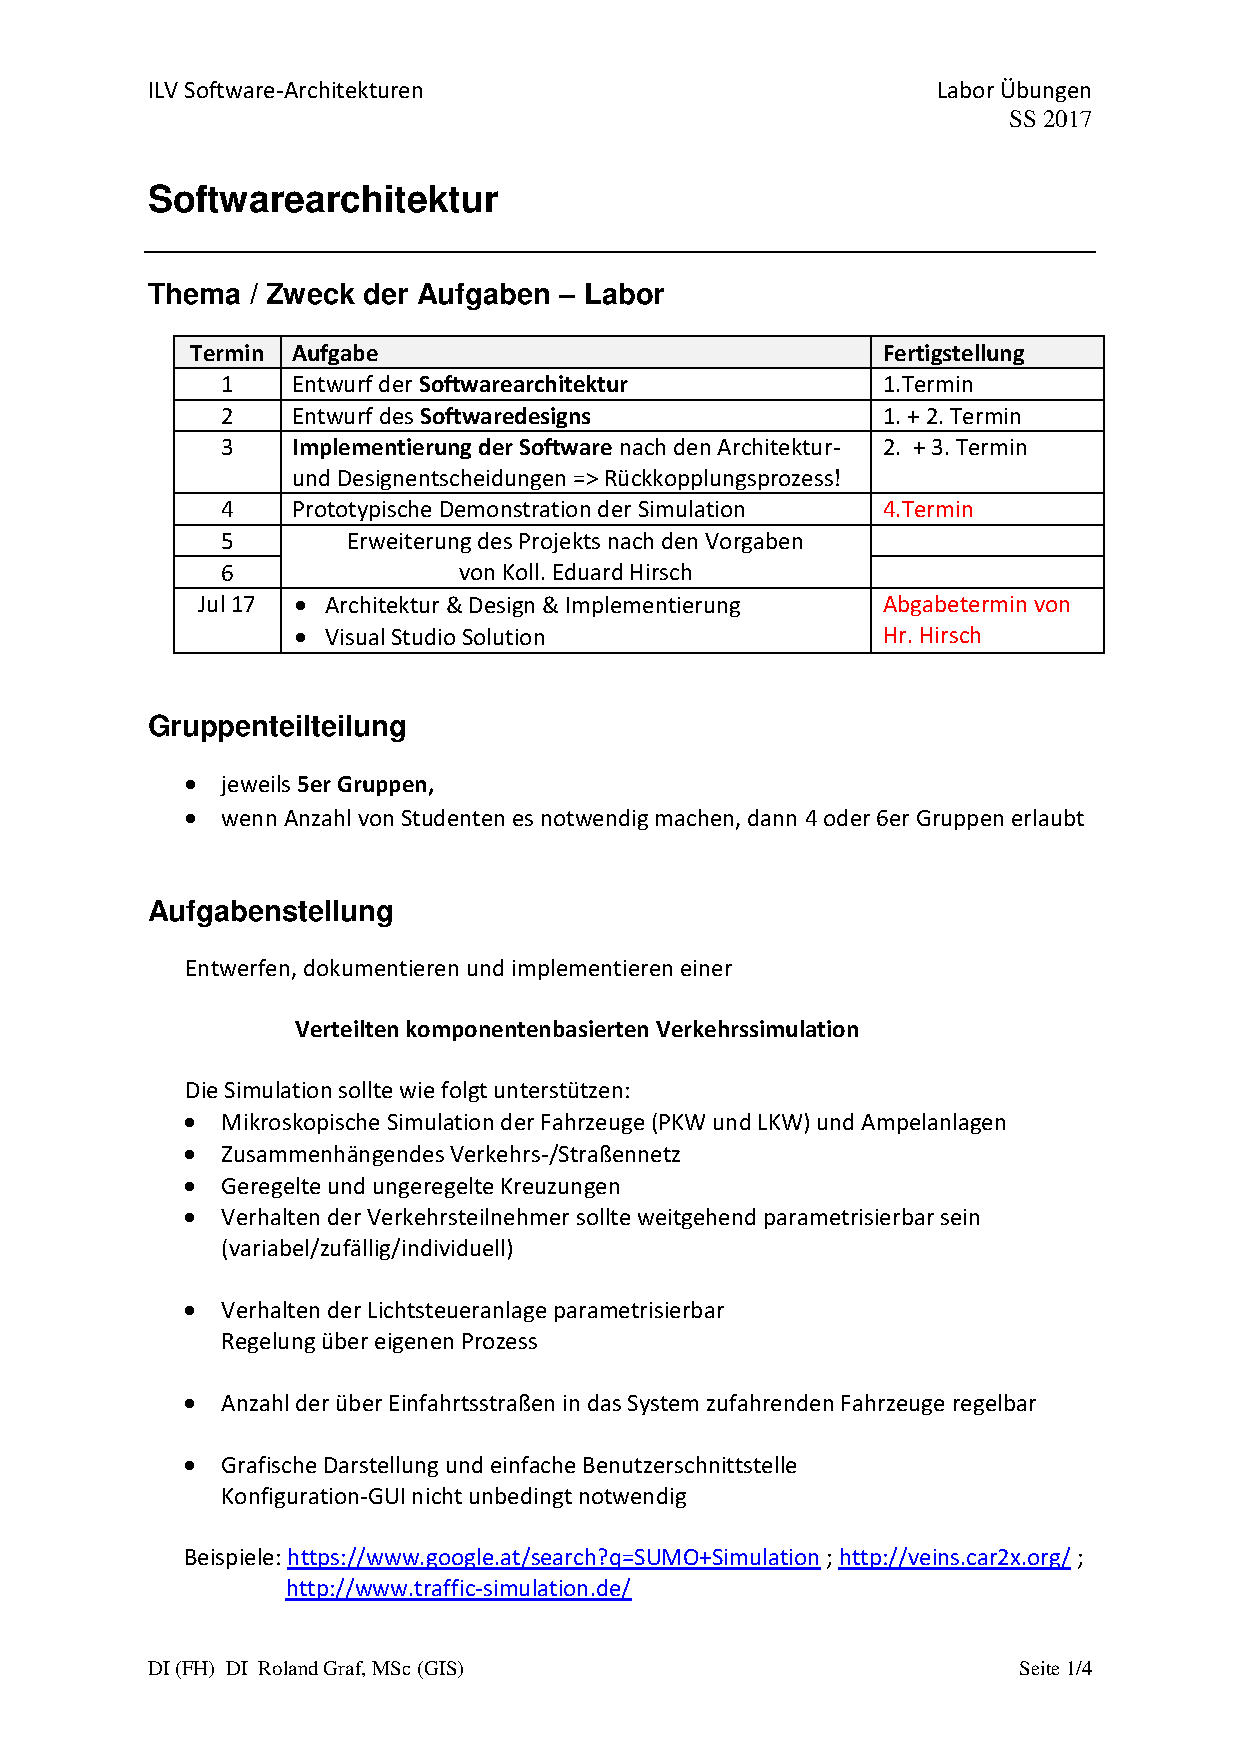
\includepdf[pages=1-4, scale=1]{Bilder/Anforderungsdokument_Verkehrsimulation.pdf}
\sloppy

\newpage



\pagebreak



% ----------------------------------------------------------------------------------------------------------
% Literatur
% ----------------------------------------------------------------------------------------------------------
\renewcommand{\centermark}{}
\renewcommand\refname{Quellenverzeichnis}
\bibliographystyle {IEEEtran}
\bibliography{bibo}

\pagebreak

%% ----------------------------------------------------------------------------------------------------------
%% Anhang
%% ----------------------------------------------------------------------------------------------------------
%
%\pagenumbering{Roman}
%\setcounter{page}{4}
%
%\lhead{Anhang \thesection}
%
%
%
%\begin{appendix}
%\section*{Anhang}
%\phantomsection
%\addcontentsline{toc}{section}{Anhang}
%\addtocontents{toc}{\vspace{-0.5em}}
%
%\section{Anhang 1}
%
%
%
%%\label{lab:anhangfem}
%%\begin{minipage}{\linewidth}
%%	\centering
%%	\includegraphics[width=1\linewidth]{Bilder/backen_stresstest.png}
%%	\captionof{figure}[Spannungsanalyse Greiferbacken]{Spannungsanalyse Greiferbacken}
%%	\label{fig:stress}
%%\end{minipage}
%%\newline
%
%\pagebreak
%
%
%
%
%%\label{lab:technKhk}
%%\begin{minipage}{\linewidth}
%%	\centering
%%	\includepdf[pages=1-1, landscape=true, scale=0.7, pagecommand={\thispagestyle{fancy}}]{pdfExtern/Keilhaken.pdf}
%%	
%%	\label{fig:technKhk}
%%\end{minipage}
%%\newline
%%\pagebreak
%
%\section{Anhang 2}
%
%\pagebreak
%
%
%%\subsection*{Screenshot}
%%\label{app:screenshot}
%%Unterkategorie, die nicht im Inhaltsverzeichnis auftaucht.
%
%
%%\subsection*{Literaturverzeichnis}
%
%%\renewcommand{\refname}{Literaturverzeichnissss}
%%%\nocite*{}%Alle anzeigen, auch die, die nicht verwendet werden
%%\bibliographystyle{plain}
%%\bibliography{bibo}{}
%
%\end{appendix}



\end{document}
